
\chapter{Interpolation newtonienne}

\section{Différences divisées et calcul du polynôme d'interpolation}

Dans toute cette partie, on notera $f$ une fonction de $\mathbb{R}$ 
dans $\mathbb{R}$ que l'on souhaite interpoler aux points 
$x_0, \dots, x_n$ (tous distincts).

On souhaite ici mettre en place un algorithme 
permettant de calculer le polynôme d'interpolation $p_n(x)$ de Lagrange 
de manière plus efficace qu'avec la base de Lagrange des polynômes
$(L_j)_{0 \leq j \leq n}$. 

\[
L_j(x) = \prod_{i = 0, i \neq k}^{n} \frac{x-x_i}{x_j -x_i}
\] 

\[
p_n(x) = \sum_{j=0}^{n} f(x_j) L_j(x)
\] 

Ce formulation a le mérite d'être très simple, mais elle 
présente un inconvénient majeur: il faut recalculer toute la 
base des polynômes lorsque l'on veut rajouter un point à 
notre interpolation. On souhaite développer une méthode qui 
n'oblige pas à recalculer entièrement le polynôme 
d'interpolation lorsqu'on ajoute un point mais qui permette 
plutôt de calculer le nouveau polynôme à partir de celui de 
degré inférieur.

\begin{definition}[Différences divisées]
Soit $f$ une fonction de  $\mathbb{R}$ dans $\mathbb{R}$ et 
$x_0, \dots, x_n$ $n+1$ points d'interpolations. On appelle 
différence divisée d'ordre $n$ la quantité notée 
$f[x_0, \dots, x_n]$ définie par 
\[
f[x_0, \dots, x_n] = \frac{f[x_1, \dots, x_n] - f[x_0, \dots, x_{n-1}]}{x_n - x_0}
\]
avec $\forall i \in \{1, \dots, n\}, f[x_i] = f(x_i)$.
\end{definition}

\begin{proposition}
La quantité $f[x_0, \dots, x_n]$ est égale au terme de degré 
$n$ dans le polynôme d'interpolation de Lagrange $p_n$ de $f$ aux points $x_0, \dots, x_n$.
\end{proposition}

\begin{proof}
On démontre le résultat par récurrence. Pour $n = 0$, la 
quantité $f[x_0]$ vaut $f(x_0)$ et correspond bien au 
polynôme d'interpolation de Lagrange. Supposons la propriété 
vraie pour $n$ points $x_0, \dots, x_{n-1}$. Notons $P$ le 
polynôme d'interpolation de Lagrange associé aux $n$ premiers 
points ($x_0, \dots, x_{n-1}$) et $Q$ celui associé aux 
$n$ derniers points ($x_1, \dots, x_{n}$). On pose
\[
L(x) = \frac{(x-x_0)Q(x) - (x-x_n)P(x)}{x_n - x_0}
\]
On a $\forall i \in \{1, \dots,n-1\}$, 
\[
L(x_i) = 
\frac{(x_i-x_0)f(x_i) - (x_i-x_n)f(x_i)}{x_n - x_0} = f(x_i)
\]
et
\[
L(x_0) = 
\frac{(x_0-x_0)Q(x_0) - (x_0-x_n)f(x_0)}{x_n - x_0} = f(x_0)
\]
\[
L(x_n) = 
\frac{(x_n-x_0)f(x_n) - (x_n-x_n)P(x_n)}{x_n - x_0} = f(x_n)
\]
Il y a donc correspondance entre $L(x)$ et le polynôme 
d'interpolation de Lagrange de degré $n$ sur $x_0, \dots, x_{n}$. On en déduit que $L$ est exactement le polynôme 
d'interpolation de Lagrange aux points $x_0, \dots, x_{n}$. 
Enfin, on constate que le terme de plus haut degré de $L$ vaut 
\[
\frac{f[x_1, \dots, x_n] - f[x_0, \dots, x_{n-1}]}{x_n - x_0}= f[x_0, \dots, x_n] 
\]
d'où le résultat.
\end{proof}


\begin{proposition}
\label{prop:interpolNewton}
Le polynôme d'interpolation de Lagrange de $f$ aux points 
$x_0, \dots, x_{n}$ peut s'écrire:
\[
p_n(x) = f[x_0] + (x-x_0)f[x_0, x_1] + \cdots + 
(x-x_0) \cdots (x-x_{n-1}) f[x_0, \dots, x_n]
\]
\end{proposition}

\begin{proof}
On démontre à nouveau le résultat par récurrence. Pour 1 points, 
le résultat est immédiat. Supposons la propriété vraie pour 
$n$ points et notons $p_{n-1}$ le polynôme d"interpolations 
de Lagrange associé. \\
Le polynôme $p_n - p_{n-1}$ s'annule en $x_0, \dots, x_{n-1}$ et 
son terme de plus haut degré vaut $f[x_0, \dots, x_n]$, on a 
donc 
\[
p_n(x) - p_{n-1}(x) = f[x_0, \dots, x_n](x-x_0) \cdots (x-x_{n-1})
\]
Soit
\begin{align*}
p_n(x) &= f[x_0, \dots, x_n](x-x_0) \cdots (x-x_{n-1}) +  p_{n-1}(x) \\
 &= f[x_0, \dots, x_n](x-x_0) \cdots (x-x_{n-1}) + 
f[x_0, \dots, x_{n-1}](x-x_0) \cdots (x-x_{n-2}) + \cdots 
+ f[x_0]
\end{align*}
ce qui montre le résultat.
\end{proof}

Cette formulation est intéressante car elle montre qu'il est 
possible de calculer les polynômes d'interpolations de manière 
récursive, en réutilisant le polynôme de degré inférieur.

\begin{remark}
La famille de polynômes $n_j$ définie par 
\[
n_j(x) = \prod_{0 \leq i < j}(x - x_i)
\]
forme une base de l'ensemble des polynômes appelée base de 
Newton.
La formule donnée dans la proposition \ref{prop:interpolNewton} est l'écriture du polynôme d'interpolation dans la base de 
Newton (d'où le nom d'interpolation newtonienne).
\end{remark}

\begin{remark}[Règle de Horner]
De la proposition \ref{prop:interpolNewton}, on déduit une 
écriture du polynôme d'interpolation permettant de réduire le
nombre de multiplication (plus rapide numériquement):
\[
p_n(x) = f[x_0] + (x-x_0)\bigg( f[x_0, x_1] + 
(x - x_1) \Big( f[x_0, x_1] + (x - x_1)(f[x_0, x_1, x_2] + \cdots) \Big) \bigg)
\]
\end{remark}

\vskip 2em

On peut facilement déduire de ce qui précède un algorithme 
permettant de calculer efficacement le polynôme d'interpolation 
de Lagrange de $f$ degré $n$ à partir de celui de degré $n-1$.

\begin{figure}[h]
  \centering
  \[
  \begin{matrix}
f(x_0) = f[x_0]&            &                & \\
               & f[x_0,x_1] &                & \\
f(x_1) = f[x_1]&            & f[x_0,x_1,x_2] & \\
               & f[x_1,x_2] &                & f[x_0,x_1,x_2,x_3]\\
f(x_2) = f[x_2]&            & f[x_1,x_2,x_3] & \\
               & f[x_2,x_3] &                & \\
f(x_3) = f[x_3]&            &                & \\
  \end{matrix}
  \]
  \caption{Pyramide du calcul des différences divisées}
  \label{fig:diffdiv}
\end{figure} 

La figure \ref{fig:diffdiv} montre qu'il est possible de 
réutiliser certains calculs de différences divisées. 
Dans notre exemple, la quantité $f[x_1,x_2]$ est en effet 
utilisé deux fois. 
On peut donc en théorie réduire le temps de calcul lorsque $n$ 
devient grand.

Le code Python donné en annexe fournit une classe \tcode{Interpolation} permettant de calculer les polynômes 
d'interpolations de Lagrange d'une fonction $f$. 
La base de Newton est utilisée pour calculer les polynômes, mais une 
méthode permettant d'effectuer le calcul en se servant de la  
base de Lagrange est également fournie à des fins 
de comparaisons. L'algorithme utilise un dictionnaire pour 
retenir les résultats de calculs des différences divisées. 


\begin{codeblock}
## Exemple d'utilisation du code Python
a = Interpolation(f) # On construit un objet permettant d'interpoler la fonction f
# On ajoute trois points d'interpolations
a.addPoint(-1)
a.addPoint(0)
a.addPoint(1)
a.P(0) # On évalue le polynôme d'interpolation en 0
a.x(1) # On récupère le deuxième point d'interpolation, ici 0
a.lagrange() # Renvoie le polynôme calculé en utilisant la base de Lagrange
\end{codeblock}


\section{Interpolation de la fonction $f(t) = \frac{1}{(1+t^2)}$}

On souhaite étudier le comportement de l'interpolation 
newtonienne sur $[-5,5]$ de la fonction $f(t) = \frac{1}{(1+t^2)}$. 

On commence dans un premier temps par utiliser des points 
d'interpolations équidistants. 
\begin{figure}[h]
  \centering
  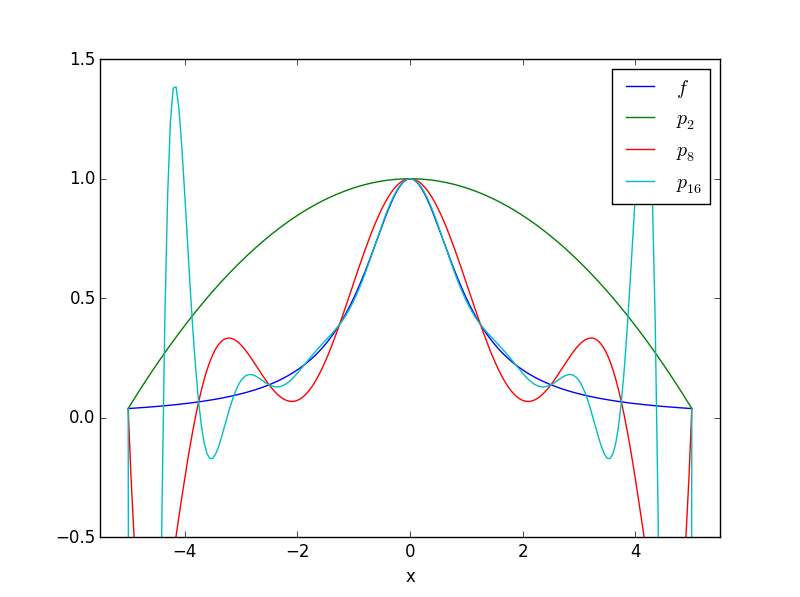
\includegraphics[scale=0.5]{fig1}
  \caption{Interpolation newtonienne avec des points équidistants}
  \label{fig:1:ptsEquidist}
\end{figure}

Comme on peut le voir dans la figure \ref{fig:1:ptsEquidist}, 
l'interpolation avec des polynômes de degré élevé semble 
être ici instable: on observe des oscillations de plus en plus 
fortes près des bords.

On peut essayer de quantifier la gravité de la situation en 
estimant numériquement la norme infinie de l'erreur à partir 
des points échantillonnés pour tracer le graphe. Les résultats 
sont donnés dans la table \ref{table:1:erreurNormInf}\footnote{Estimé sur la base de 240 points répartis uniformément sur $[-5,5]$.}.

\begin{table}[h]
  \centering
\begin{tabular}{cccccccc}
     & $p_1$ & $p_2$ & $p_3$ & $p_4$ & $p_8$ & $p_{16}$ & $p_{32}$ \\
   Erreur & 0.962 & 0.646 & 0.707 & 0.438 & 1.045 & 14.32 & 4777.995\\
\end{tabular}
  \caption{Norme infinie de $|p_n-f|$}
  \label{table:1:erreurNormInf}
\end{table}


Pour améliorer les résultats, on peut interpoler aux points 
de Tchebychev definis par 
\[
x_k = \cos\left( \frac{2k-1}{2n} \pi \right), \quad k = 1, \dots n
\]
Ces points sont définis pour une interpolation sur l'intervalle 
$[-1, 1]$ mais il est facile de leur appliquer une transformation 
pour un intervalle quelconque $[a, b]$.
\[
x_k = \frac{1}{2}(a+b) +\frac{1}{2}(b-a)\cos\left( \frac{2k-1}{2n} \pi \right), \quad k = 1, \dots n
\]

On obtient dans ce cas une interpolation plus stable que précédemment (c.f. figure \ref{fig:1:ptsTcheby}).

\begin{figure}[h]
  \centering
  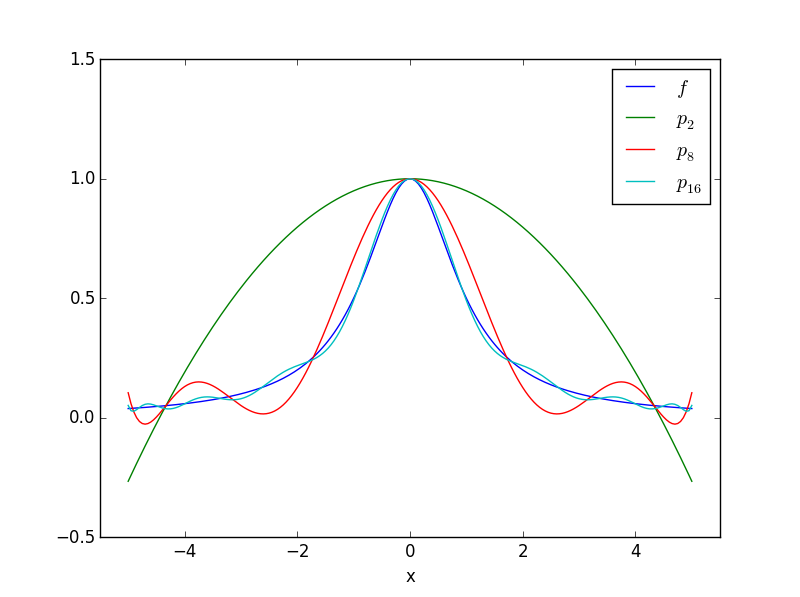
\includegraphics[scale=0.5]{fig2}
  \caption{Interpolation newtonienne avec les points de Tchebychev}
  \label{fig:1:ptsTcheby}
\end{figure}


\section{Interpolation de la fonction $g(x) = 2(1+\tanh(x)) - x/10 $}

On considère cette fois la fonction $g(x) = 2(1+\tanh(x)) - \frac{x}{10}$ sur $[-6, 6]$. 

Les figures \ref{fig:2:ptsUniform} et \ref{fig:2:ptsTcheby} montre 
le graphe de $g$ et du polynôme d'interpolation de Lagrange avec 
des points d'interpolations équidistants et de Tchebychev.

\begin{figure}[h]
  \centering
  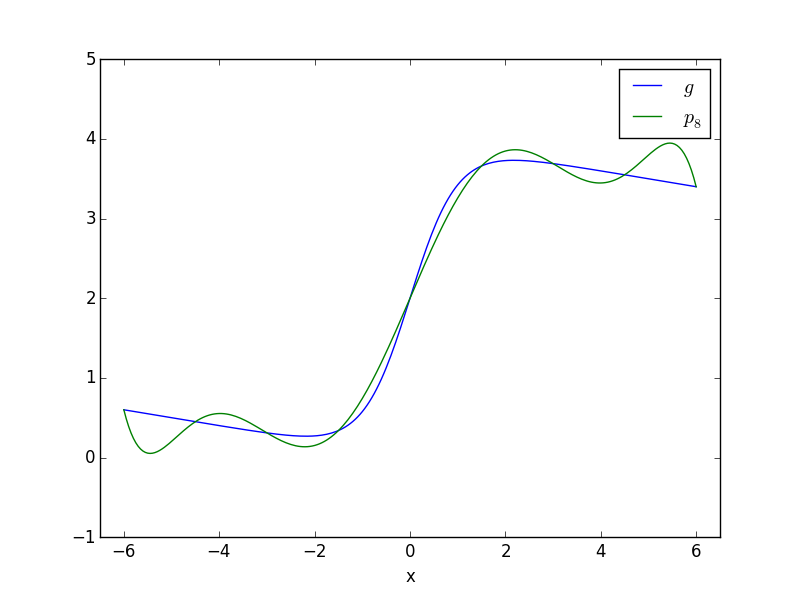
\includegraphics[scale=0.5]{fig3}
  \caption{Interpolation avec 9 points équidistants}
  \label{fig:2:ptsUniform}
\end{figure}


\begin{figure}[h]
  \centering
  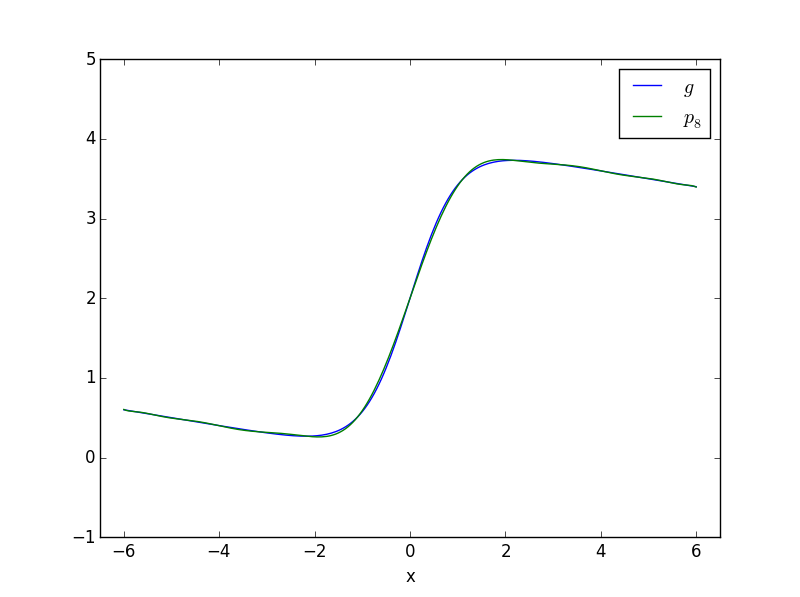
\includegraphics[scale=0.5]{fig4}
  \caption{Interpolation avec les 9 points de Tchebychev}
  \label{fig:2:ptsTcheby}
\end{figure}

On constate comme précédemment que les points de Tchebychev 
donnent de meilleurs résultats. 

Un autre point intéressant est que la fonction que l'on 
interpole présente une anti-symétrie, i.e.\ $g(x) = -g(-x)$; 
et que nos deux polynômes d'interpolations présentent également 
cette même propriété. Ainsi, l'erreur commise au point $x$ est 
égale à l'opposé de l'erreur commise en $-x$. Cela signifie que 
si l'on intègre sur l'intervalle complet, l'erreur est en moyenne 
nulle. Autrement dit, notre polynôme d'interpolation peut être 
utilisé pour calculer de manière exacte l'intégrale de $g$.

On peut constater cela avec le code suivant.

\begin{codeblock}
import scipy.integrate as integrate
i1 = integrate.quad(g, xmin, xmax)
P = a.P.integ() # a est notre objet de type Interpolation
i2 = P(xmax) - P(xmin)
print(i1, i2)
\end{codeblock}

Une sortie possible de ce programme est:
\begin{codeblock}
(23.999999999999996, 2.664535259100375e-13) 24.0
\end{codeblock}
Le couple correspond à un calcul numérique de l'intégrale et 
une borne pour l'erreur commise; le dernier nombre correspond 
à la valeur de l'intégrale calculée à partir du polynôme 
d'interpolation.


\section{Comparaison avec l'interpolation lagrangienne}

On se propose dans cette partie d'effectuer quelques mesures 
pour comparer l'efficacité des différents algorithmes.

Un programme en Python a été écrit pour comparer le temps mis 
pour calculer le polynôme d'interpolation en utilisant la 
base de Newton et la base de Lagrange. La fonction à interpoler 
est le cosinus, et les points d'interpolations sont tirés au hasard 
dans l'intervalle $[-1, 1]$. On tire $N$ points et l'on calcule 
le polynôme d'interpolation en utilisant une base puis l'autre. 
On mesure le temps mis pour faire le calcul dans chacune des bases.

Le tableau \ref{table:compNewtonLagrange} montre les résultats 
pour différentes valeurs de $N$. On constate assez clairement 
un avantage pour la base de Newton. 
Attention cependant, cette avantage est dû à l'utilisation d'un 
cache pour le calcul des différences divisées : sans ce cache, 
le coût du calcul des différences divisées augmente de manière 
exponentielle et rend la méthode inutilisable.
Enfin, ces 
mesures sont à prendre avec précaution, les algorithmes n'ayant pas 
été particulièrement optimisés.

\begin{table}[h]
  \centering
\begin{tabular}{ccccccccccc}
    $N$ & 10 & 20 & 30 & 40 & 50 & 60 & 70 & 80 & 90 & 100 \\
   Lagrange (s) & 0.032 & 0.113 & 0.246 & 0.423 & 0.654 & 0.953 & 1.286 & 1.716 & 2.142 & 2.640 \\
   Newton (s) & 0.015 & 0.049 & 0.094 & 0.165 & 0.244 & 0.353 & 0.484 & 0.627 & 0.782 & 0.965 \\
\end{tabular}
  \caption{Efficacité des différentes méthodes de calculs}
  \label{table:compNewtonLagrange}
\end{table}



\chapter{Interpolation polynomiale par morceau : splines}

\section{Définition d'une spline }

Dans toute cette partie, on notera $f$ une fonction de $\mathbb{R}$ 
dans $\mathbb{R}$ que l'on souhaite interpoler aux points 
$x_0, \dots, x_n$ (tous distincts).

On souhaite ici mettre en place un algorithme 
permettant de calculer une fonction d'interpolation $s$ dite "spline"

\begin{definition}[Fonction spline]
Soit $s$ une fonction de à valeurs dans $\mathbb{R}$ et 
$x_0, \dots, x_n$ $n+1$ points d'interpolations. $s$ est une spline de degré $n$ si elle respecte
ces deux propriétés :
\begin{enumerate}
\item Les valeurs de $f$ aux points $x_0, \dots, x_n$ est respectée
\item La fonction $s$ est continue et ses dérivées d-ièmes également pour pour $d$ allant de $0$ à $n-1$
\item La fonction $s$ est polynomiale de degré n sur les intervalles $[x_i,x_{i+1}]$ pour $i$ allant de $0$ à $n-1$
\end{enumerate}
\end{definition}

On se place maintenant sur un intervalle $[x_i,x_{i+1}]$ avec $i$ fixé entre 0 et $n-1$ et dans le cas d'une spline cubique ($d = 3$)
En dérivant deux fois, on obtient avec la troisième propriété :
\[
s''(x) = \frac{(x_{i+1} - x)M_i + (x - x_i)M_{i+1}}{h_i}
\]
avec $h_i = x_{i+1} - x_i$, $M_i = s''(x_i)$. On connaît donc les $(h_i)_i$ mais les $(M_i)_i$ restent des inconnus

En intégrant successivement deux fois on obtient les trois formulations suivantes:
\[
s''(x) = \frac{(x_{i+1} - x)M_i + (x - x_i)M_{i+1}}{h_i}
\]
\[
s'(x) = \frac{-(x_{i+1} - x)^{2}M_i + (x - x_i)^{2}M_{i+1}}{2h_i} + A_i
\]
\[
s(x) = \frac{(x_{i+1} - x)^{3}M_i + (x - x_i)^{3}M_{i+1}}{6h_i} + C_i(x_{i+1}-x) +D_i(x-x_i)
\]
avec $A_i = D_i - C_i$, et on note de plus $y_i = f(x_i)$. Ainsi on obtient une expression des inconnues C_i et D_i
en fonction des M_i à partir de la première propriété de la définition (les valeurs aux points de subdivision).
\[
C_i = \frac{y_i}{h_i} - \frac{h_iM_i}{6}
\]
\[
D_i = \frac{y_{i+1}}{h_i} - \frac{h_iM_{i+1}}{6}
\]

Il ne nous reste donc plus qu'à calculer les $(M_i)_i$ pour avoir une expression explicite de notre spline.
Pour celà, on utilise la continuité de $s'$ aux points de subdivision et on obtient pour le point $x_{i}$ pour i allant de 1 à $n-1$ donc :
\[
\frac{h_{i-1}M_{i}}{2} + A_{i-1} = \frac{h_{i}M_{i}}{2} + A_{i}
\]
Soit
\[
{M_{i}} = 2\frac{A_{i}-A_{i-1}}{h_{i}-h_{i-1}}
\]
En développant les $A_{i-1}$ et $A_{i}$ on obtient finalement
\[
\frac{2}{3}M_{i} +\frac{h_{i+1}}{3(h_{i-1}+h_{i})}M_{i+1}+\frac{h_{i}}{3(h_{i-1}+h_{i})}M_{i-1} = \frac{2}{h_{i-1}+h_{i}} (\frac{y_{i+1} - y_{i}}{h_{i}} - \frac{y_{i} - y_{i-1}}{h_{i-1}})
\]
De même, en prenant la continuité au point $x_i$, on obtient pour i allant de 1 à $n-1$.
Il nous manque alors deux équations pour pouvoir déterminer les $(M_i)_i$,
ces dernières vont êtres données par les conditions limites aux points $x_0$ et $x_n$.
Il ne restera plus alors qu'à resoudré un système linéaire que nous pouvons rentrer sous forme d'un système matriciel $AM = B$
avec M le vecteur colonne des $(M_i)_i$
Au vu des équations, on remarque que le calcul est beaucoup plus simple avec des points équidistants (et donc égalité des $(h_i)_i$)

\section{Cas d'une spline naturelle}

\begin{definition}[Spline naturelle]
On appelle une $s$ une spline naturelle si $s$ est une spline et que
son accélération au bord de son intervalle de définition est nulle.
\end{definition}

Dans ce cas, la résolution du système linéaire évoqué précédemment est simple,
les condition nous donnent $M_0$ et $M_n$ et on obtient la matrice tridiagonale
A suivante pour calculer Les $M_i$ aux points intérieurs:
\[
\begin{bmatrix}
    2/3 & h_1/3(h_0+h_1) & 0 & 0 & \dots  & 0 \\
    h_2/3(h_1+h_2) & 2/3 & h_3/3(h_1+h_2) & 0 & \dots  & 0 \\
    0 &  h_3/3(h_2+h_3) & 2/3 & h_4/3(h_2+h_3) & \dots & 0 \\
    \vdots & \ddots & \ddots & \ddots & \ddots \\
    0 & \dots & 0 & h_{n-2}/3(h_{n-3}+h_{n-2}) & 2/3 & h_{n-1}/3(h_{n-3}+h_{n-2}) \\
    0 & \dots & 0 & 0 & h_{n-1}/3(h_{n-2}+h_{n-1}) & 2/3
\end{bmatrix}
\]
Et la matrice B défini par $b_i =  \frac{2}{h_{i-1}+h_{i}} (\frac{y_{i+1} - y_{i}}{h_{i}} - \frac{y_{i} - y_{i-1}}{h_{i-1}})$.
On note par ailleurs que si les points sont équidistants, la matrice A est symétrique et de termes constants sur ses trois diagonales.

\section{Convergence d'une spline}
\begin{proposition}[Convergence en norme infinie]
Soit $f$ une fonction continue de $[a,b]$ à valeurs dans $\mathbb{R}$ et $(X_n)_n$ une famille de subdivision de $[a,b]$ telle que
$\lim\limits_{n \rightarrow +\infty} \delta(X_n) =  0$. Alors on a convergence en norme infinie de la suite des splines $(s_n)_n$ interpolées
pour les subdivisions $X_n$ vers $f$.
Avec $\delta(X_n)$ la distance maximale séparant deux points de la subdivision $X_n$
\end{proposition}

Nous allons vérifier visualiser cette proposition en prenant pour exemple la fonction $f$ définie par:

$f(x) = 2(1 + tanh(x)) - x/10$ sur l'intervalle $[-6,+6]$.
\begin{figure}[h]
  \centering
  \begin{subfigure}[b]{0.4\linewidth}
    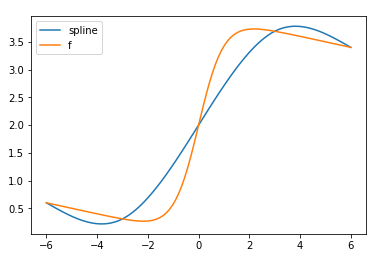
\includegraphics[width=\linewidth]{fig5}
    \caption{Avec 5 points}
  \end{subfigure}
  \begin{subfigure}[b]{0.4\linewidth}
    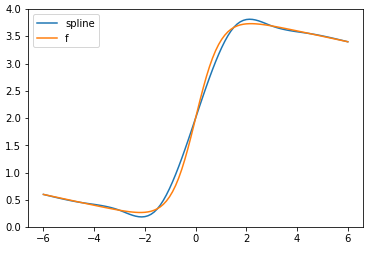
\includegraphics[width=\linewidth]{fig6}
    \caption{Avec 9 points}
  \end{subfigure}
  \begin{subfigure}[b]{0.4\linewidth}
    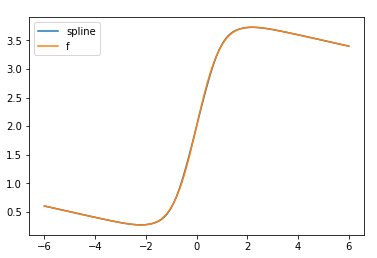
\includegraphics[width=\linewidth]{fig7}
    \caption{Avec 15 points}
  \end{subfigure}
  \begin{subfigure}[b]{0.4\linewidth}
    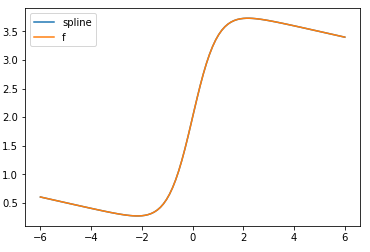
\includegraphics[width=\linewidth]{fig8}
    \caption{Avec 90 points}
  \end{subfigure}
  \caption{Interpolation de la fonction par spline avec différents nombre de points équidistants}
  \label{fig:6:fspl}
\end{figure}

L'avantage de la convergence en norme infinie est qu'elle est très visuelle. Et on voit bien à l'aide de ces figures que la convergence est très rapide \ref{fig:6:fspl}.
Avec 15 points, le résultat est déjà très satisfaisant et donne (visuellement) le même rendu qu'en le faisant avec 90 points.
La courbe obtenue avec les 9 points d'interpolation nous permet de comprendre les limites de la méthode (pour un nombre faible de points en tout cas).
On voit que sur l'intervalle $[-2,+2]$, la spline approche moins bien la fonction que sur le reste; en dehors des points de subdivision facilement repérables car
points sécants des coubes.

Si on se repenche sur les calculs de la section précédente, on constate que le vecteur B correspond à une approximation de la dérivée seconde aux
points de subdivision. La matrice A est dans notre cas symétrique et le terme dominant sur chaque ligne est celui de la diagonale principale. On a donc
une grande corrélation entre la dérivée seconde de la fonction $f$ et les termes $M_i$. Ainsi en prenant la dérivée troisième de notre spline constant égale à
$\frac{M_{i+1} - M_i}{h_i}$, ce qui nous donne grossièrement une approximation de la dérivée troisième de $f$. Ainsi si la dérivée troisième de $f$ varie,
la non-continuité de la dérivée troisième de notre fonction spline sera de plus en plus importante alors que la fonction que nous souhaitons interpoler est ici
infiniment dérivable (et de dérivées continues) sur tout l'intervalle. Les constantes apportées par continuité des premières dérivées ($C_i$ et $D_i$) qui
n'interviennent pas dans la dérivée troisième vont assurer les raccordements aux points de subdivision mais celà entraîne des mauvaises approximations
de la dérivée première en ces points.

\begin{table}[h]
  \centering
\begin{tabular}{cccccccccccc}
    $N$ & 5 & 6 & 7 & 9 & 10 & 12 & 15 & 20 & 25 & 30 & 45  \\
   Erreur & 0.715 & 0.199 & 0.392 & 0.210 & 0.014 & 0.006 & 0.032 & 0.005 & 0.002 & 0.001 & 0.0001 \\
\end{tabular}
  \caption{Erreur en norme infinie en fonction du nombre de points d'interpolation}
  \label{table:errspl}
\end{table}

Pour vérifier le bon fonctionnement de la méthode et de l'algorithme, on peut tester avec une fonction de dérivée troisième nulle,
c'est-à-dire une fontion polynomiale de degré 2. Avec des points équidistants, le calcul littéral nous donne pour tout $i$ allant de
1 à $n-1$, $b_i = 2$ puis $M_i = 2a$. avec a le coefficient de degré 2 de la fonction $f$. On obtient alors $s''(x) = 2a$ donc $s$ et $f$
ont des dérivées secondes égales et les valeurs aux points $x_i$ et $x_{i+1}$ nous assurent que $s$ et $f$ sont égales.

\begin{figure}[h]
  \centering
  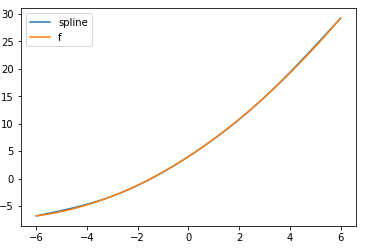
\includegraphics[scale=1.0]{fig9}
  \caption{Interpolation spline d'un polynôme de degré 2 avec 5 points}
  \label{fig:7:noerr}
\end{figure}

On constate néanmoins que la spline déterminées par l'algorithme n'est pas strictement égale à la fonction $f$ \ref{fig:7:noerr}. Néanmoins, si on compare avec l'interpolation obtenue avec le même nombre de points, le résultat est bien meilleur. La légère erreure est peut être supputable à des approximations de calculs en base binaire ou à la méthode de résolution du système linéaire.

A l'inverse, on peut tester avec une autre fonction plus semblable au premier exemple où les dérivées sont importantes $f(x) = arctan(x^3)$
\begin{figure}[h]
  \centering
  \begin{subfigure}[b]{0.4\linewidth}
    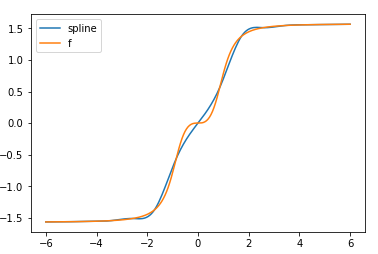
\includegraphics[width=\linewidth]{fig12}
    \caption{Avec 15 points}
  \end{subfigure}
  \begin{subfigure}[b]{0.4\linewidth}
    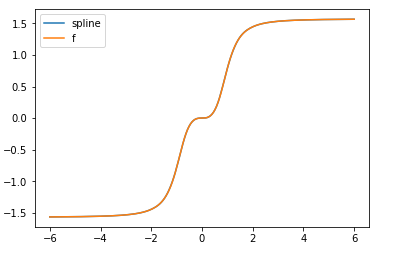
\includegraphics[width=\linewidth]{fig13}
    \caption{Avec 30 points}
  \end{subfigure}
  \caption{Interpolation de la fonction par spline avec différents nombre de points équidistants}
  \label{fig:8:fspl2}
\end{figure}

On retrouve bien les mêmes caractéristiques pour les erreurs que pour le premier exemple \ref{fig:6:fspl}. Pour améliorer l'approximation,
il y a deux possibbilités :
\begin{enumerate}
\item Augmenter le nombre de points dans la subdivision
\item Augmenter le degré de la spline
\end{enumerate}
BIen évidemment, la première solution ralonge le temps de calcul, notamment pour le système matriciel de taille $(n-1)^2$ et nous assure la convergence
uniforme. Pour la deuxième solution, de même qu'une spline cubique est limitée pour les fonctions à dérivée troisème importante, augmenter le degré
est utile qu'on finira par tomber sur une dérivée à faibles valeurs, d'autant plus qu'augmenter le nombre de degré sans augmenter le nombre de points
diminue l'exactitude des termes dérivés approximés dans la matrice $B$. Et augmenter le degré de la matrice va alourdir la matrice (mais pas en taille
comme la première méthode), diminuant son conditionnement et les méthodes de résolutions numériques.